\begin{figure}
	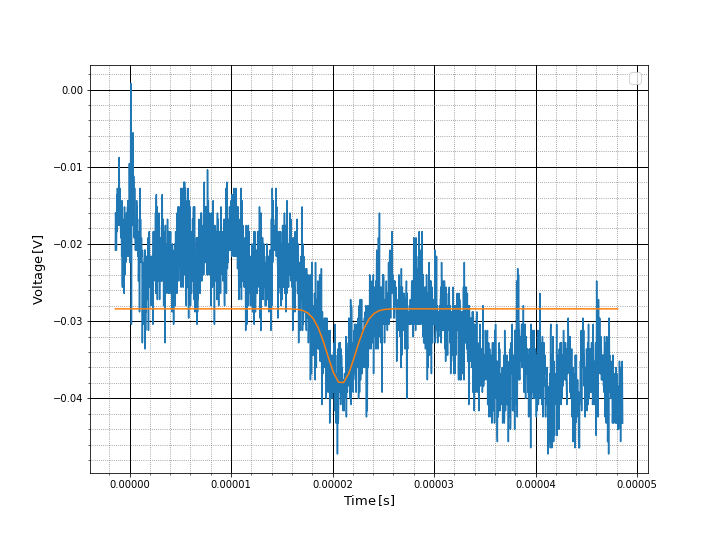
\includegraphics[scale=0.5]{Bild/S1}
	\centering
	\caption[Gaußfit an Messung bei Konst. Spannung 1]{Gaußfit an die Messungen der Elektronenwolken bei einer Spannung von $48\,$V und einem Abstand zwischen Nadel und Lase von $10.6$\,mm.}
\end{figure}
\begin{figure}
	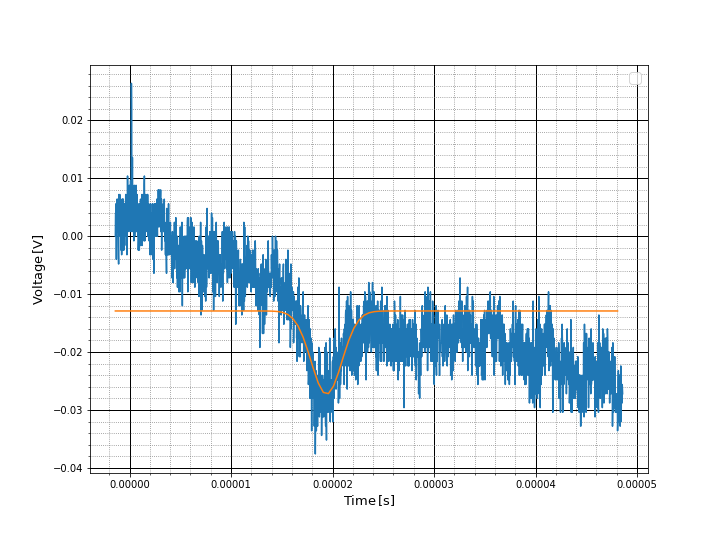
\includegraphics[scale=0.5]{Bild/S2}
	\centering
	\caption[Gaußfit an Messung bei Konst. Spannung 2]{Gaußfit an die Messungen der Elektronenwolken bei einer Spannung von $48\,$V und einem Abstand zwischen Nadel und Lase von $9.6$\,mm.}
\end{figure}
\begin{figure}
	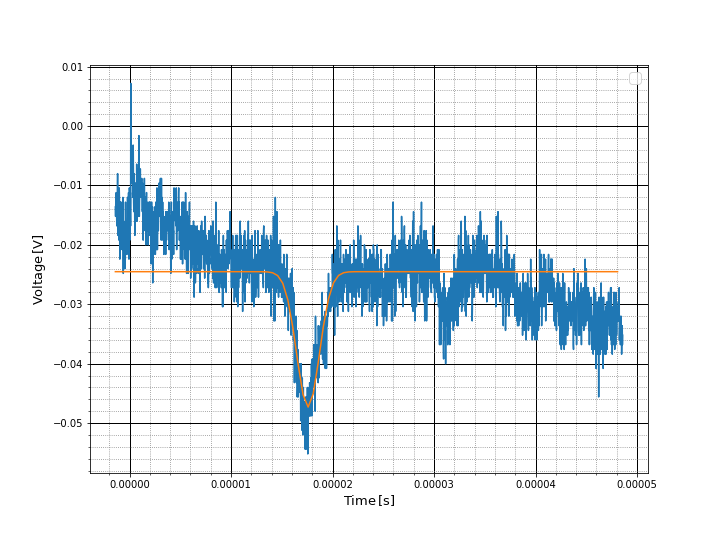
\includegraphics[scale=0.5]{Bild/S3}
	\centering
	\caption[Gaußfit an Messung bei Konst. Spannung 3]{Gaußfit an die Messungen der Elektronenwolken bei  einer Spannung von $48\,$V und einem Abstand zwischen Nadel und Lase von $8.6$\,mm.}
\end{figure}
\begin{figure}
	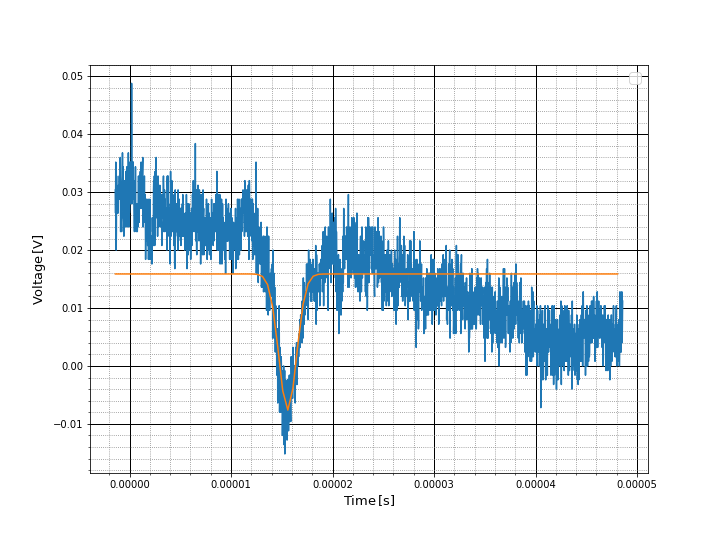
\includegraphics[scale=0.5]{Bild/S4}
	\centering
	\caption[Gaußfit an Messung bei Konst. Spannung 4]{Gaußfit an die Messungen der Elektronenwolken bei  einer Spannung von $48\,$V und einem Abstand zwischen Nadel und Lase von $7.6$\,mm.}
\end{figure}
\begin{figure}
	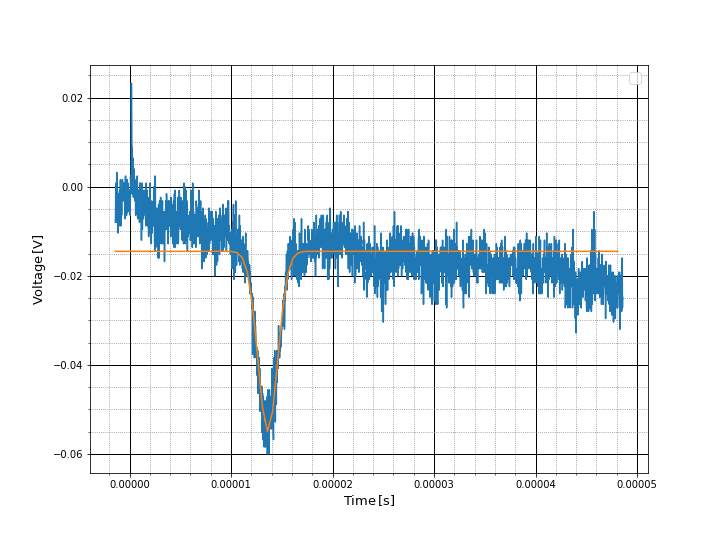
\includegraphics[scale=0.5]{Bild/S5}
	\centering
	\caption[Gaußfit an Messung bei Konst. Spannung 5]{Gaußfit an die Messungen der Elektronenwolken bei einer Spannung von $48\,$V und einem Abstand zwischen Nadel und Lase von $6.6$\,mm.}
\end{figure}
\begin{figure}
	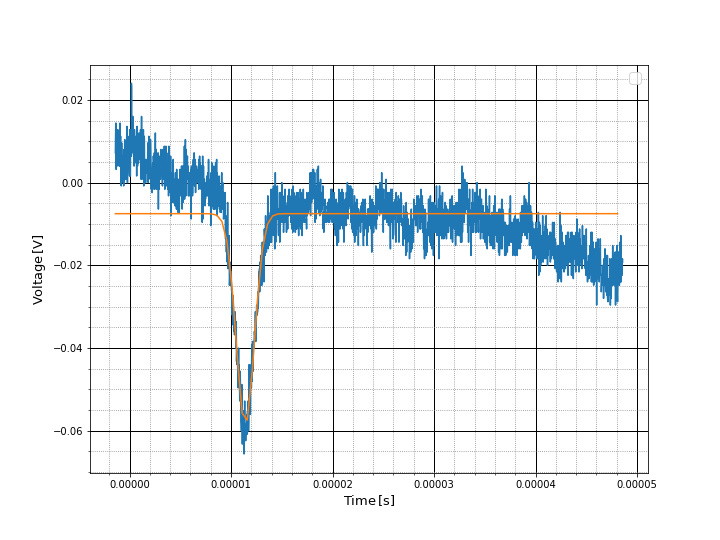
\includegraphics[scale=0.5]{Bild/S6}
	\centering
	\caption[Gaußfit an Messung bei Konst. Spannung 6]{Gaußfit an die Messungen der Elektronenwolken bei einer Spannung von $48\,$V und einem Abstand zwischen Nadel und Lase von $5.6$\,mm.}
\end{figure}
\begin{figure}
	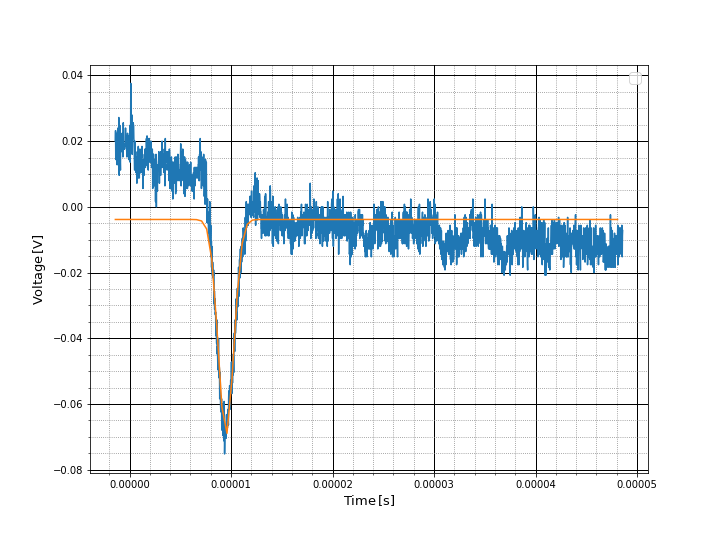
\includegraphics[scale=0.5]{Bild/S7}
	\centering
	\caption[Gaußfit an Messung bei Konst. Spannung 7]{Gaußfit an die Messungen der Elektronenwolken bei einer Spannung von $48\,$V und einem Abstand zwischen Nadel und Lase von $4.6$\,mm.}
\end{figure}
\begin{figure}
	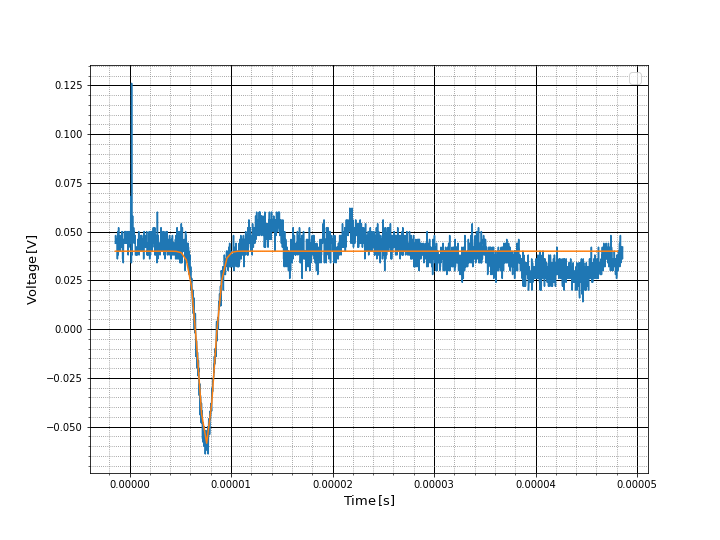
\includegraphics[scale=0.5]{Bild/S8}
	\centering
	\caption[Gaußfit an Messung bei Konst. Spannung 8]{Gaußfit an die Messungen der Elektronenwolken bei einer Spannung von $48\,$V und einem Abstand zwischen Nadel und Lase von $3.6$\,mm.}
\end{figure}

%Andere Messreihe

\begin{figure}
	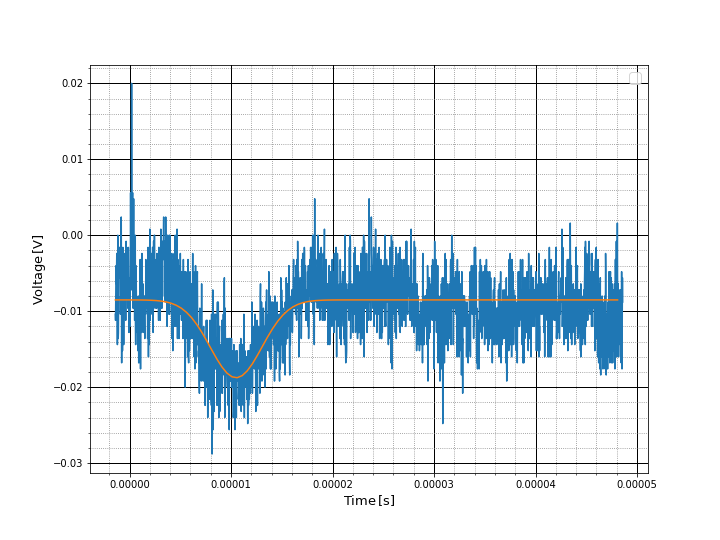
\includegraphics[scale=0.5]{Bild/A1}
	\centering
	\caption[Gaußfit an Messung bei Konst. Abstand]{Gaußfit an die Messungen der Elektronenwolken bei Konstantem Abstand von $3.6$\,mm und einer Spannung von $-13.2$\,V}
\end{figure}
\begin{figure}
	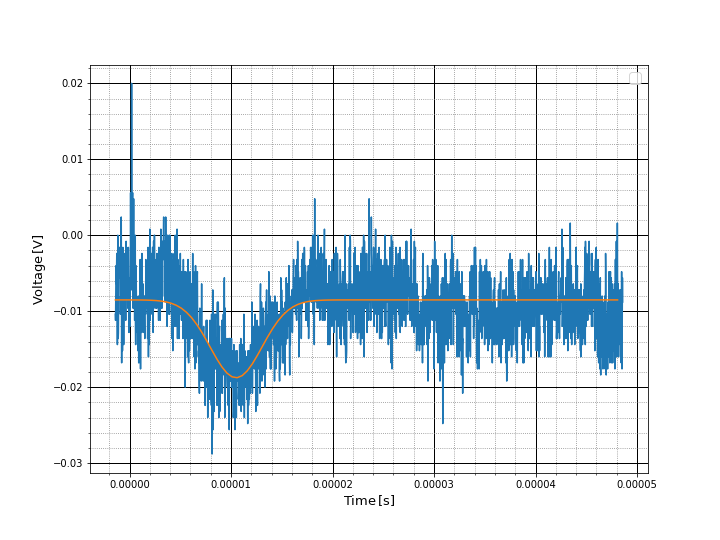
\includegraphics[scale=0.5]{Bild/A1}
	\centering
	\caption[Gaußfit an Messung bei Konst. Abstand]{Gaußfit an die Messungen der Elektronenwolken bei Konstantem Abstand von $3.6$\,mm und einer Spannung von $-15.2$\,V}
\end{figure}
\begin{figure}
	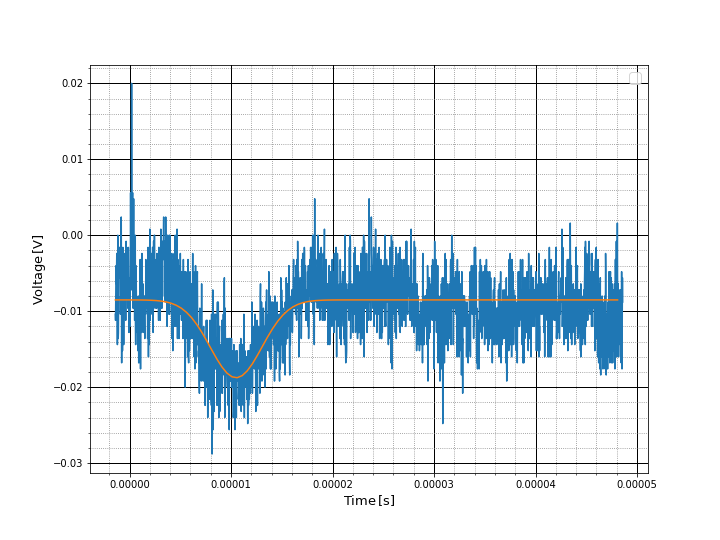
\includegraphics[scale=0.5]{Bild/A1}
	\centering
	\caption[Gaußfit an Messung bei Konst. Abstand]{Gaußfit an die Messungen der Elektronenwolken bei Konstantem Abstand von $3.6$\,mm und einer Spannung von $-18.4$\,V}
\end{figure}
\begin{figure}
	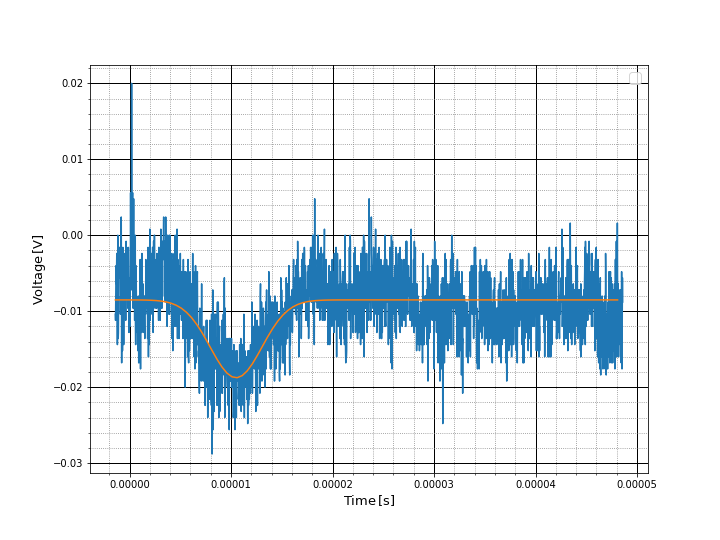
\includegraphics[scale=0.5]{Bild/A1}
	\centering
	\caption[Gaußfit an Messung bei Konst. Abstand]{Gaußfit an die Messungen der Elektronenwolken bei Konstantem Abstand von $3.6$\,mm und einer Spannung von $-20.4$\,V}
\end{figure}
\begin{figure}
	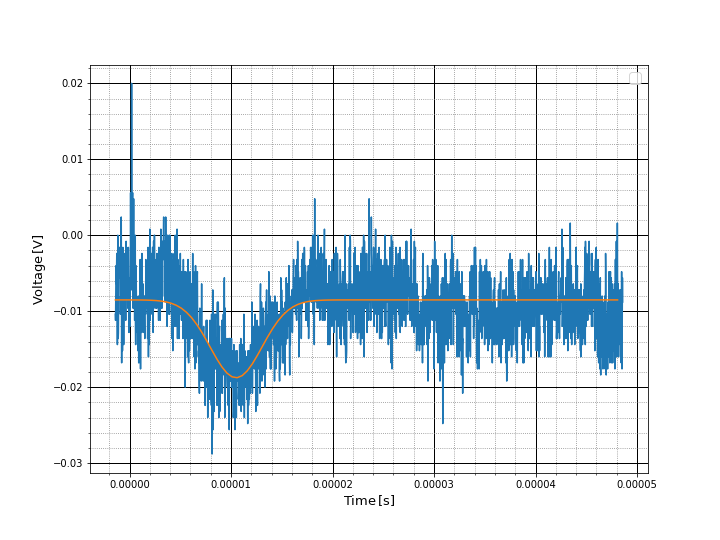
\includegraphics[scale=0.5]{Bild/A1}
	\centering
	\caption[Gaußfit an Messung bei Konst. Abstand]{Gaußfit an die Messungen der Elektronenwolken bei Konstantem Abstand von $3.6$\,mm und einer Spannung von $-22.4$\,V}
\end{figure}
\begin{figure}
	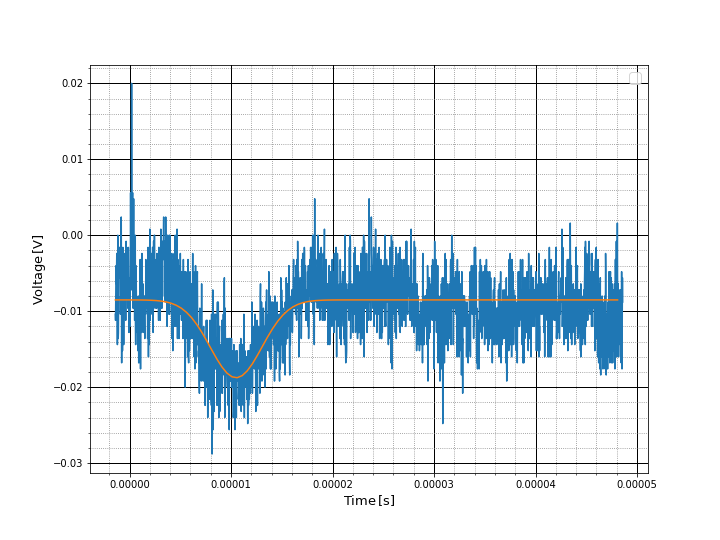
\includegraphics[scale=0.5]{Bild/A1}
	\centering
	\caption[Gaußfit an Messung bei Konst. Abstand]{Gaußfit an die Messungen der Elektronenwolken bei Konstantem Abstand von $3.6$\,mm und einer Spannung von $-24.4$\,V}
\end{figure}
\begin{figure}
	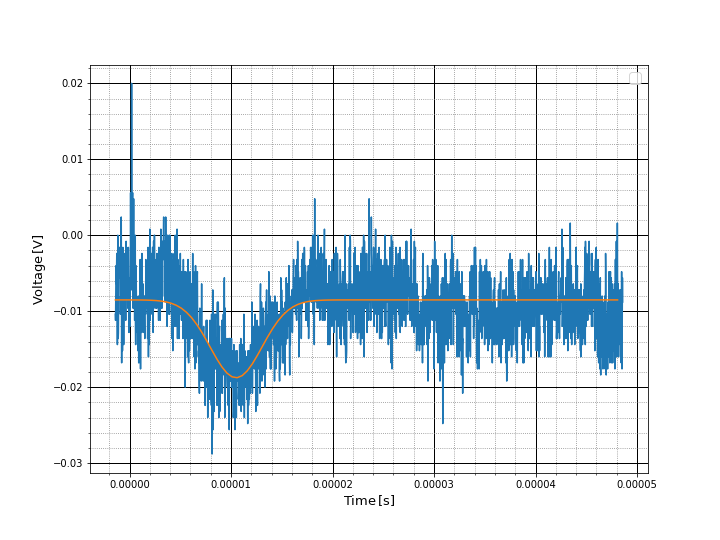
\includegraphics[scale=0.5]{Bild/A1}
	\centering
	\caption[Gaußfit an Messung bei Konst. Abstand]{Gaußfit an die Messungen der Elektronenwolken bei Konstantem Abstand von $3.6$\,mm und einer Spannung von $-28.0$\,V}
\end{figure}
\begin{figure}
	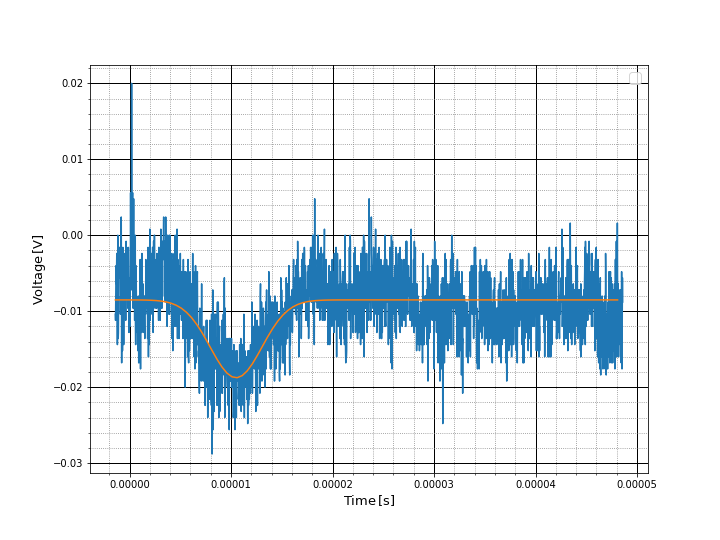
\includegraphics[scale=0.5]{Bild/A1}
	\centering
	\caption[Gaußfit an Messung bei Konst. Abstand]{Gaußfit an die Messungen der Elektronenwolken bei Konstantem Abstand von $3.6$\,mm und einer Spannung von $-32.0$\,V}
\end{figure}
\begin{figure}
	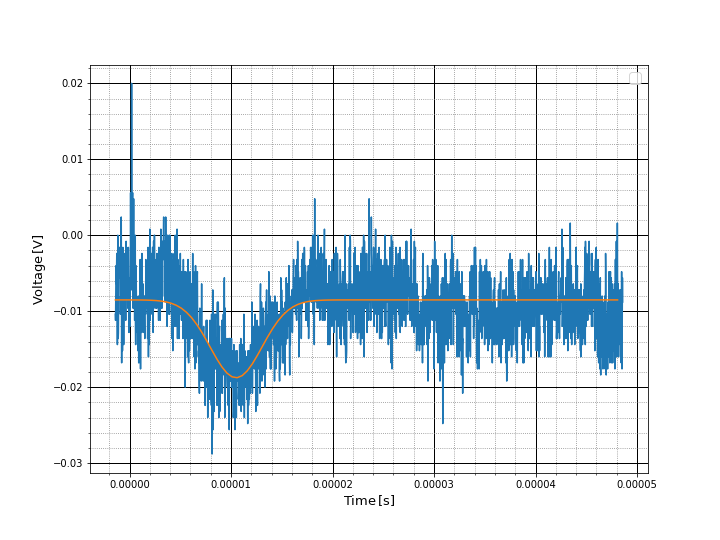
\includegraphics[scale=0.5]{Bild/A1}
	\centering
	\caption[Gaußfit an Messung bei Konst. Abstand]{Gaußfit an die Messungen der Elektronenwolken bei Konstantem Abstand von $3.6$\,mm und einer Spannung von $-36.0$\,V}
\end{figure}
\begin{figure}
	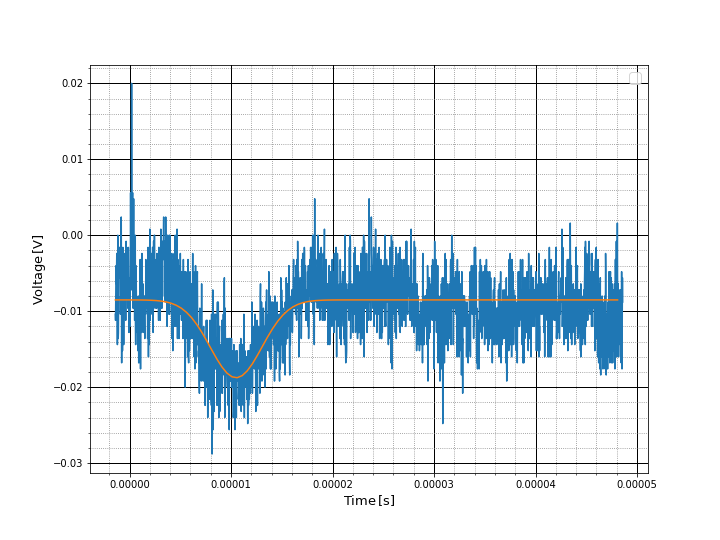
\includegraphics[scale=0.5]{Bild/A1}
	\centering
	\caption[Gaußfit an Messung bei Konst. Abstand]{Gaußfit an die Messungen der Elektronenwolken bei Konstantem Abstand von $3.6$\,mm und einer Spannung von $-40.0$\,V}
\end{figure}
\begin{figure}
	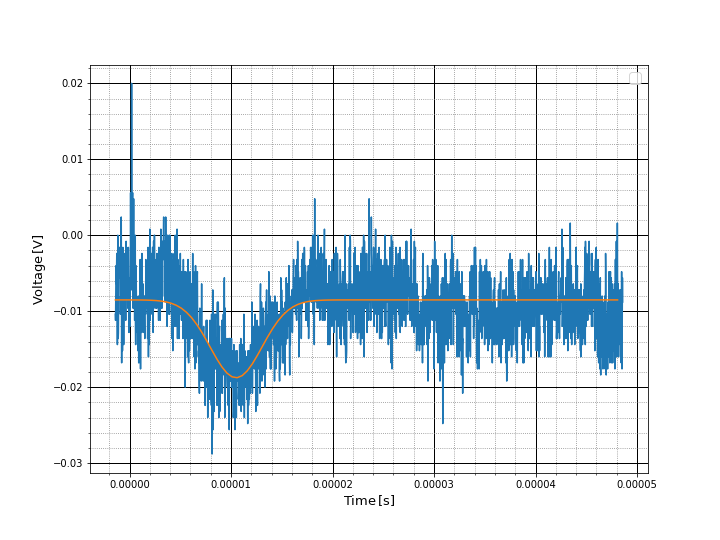
\includegraphics[scale=0.5]{Bild/A1}
	\centering
	\caption[Gaußfit an Messung bei Konst. Abstand]{Gaußfit an die Messungen der Elektronenwolken bei Konstantem Abstand von $3.6$\,mm und einer Spannung von $-44.0$\,V}
\end{figure}
\begin{figure}
	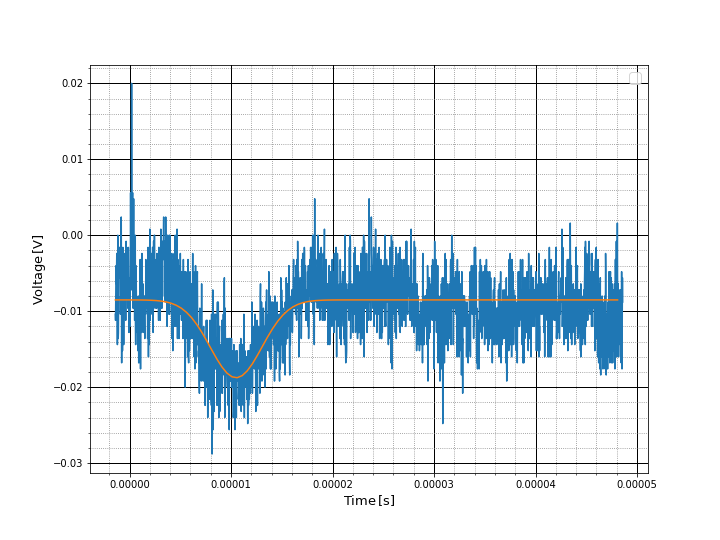
\includegraphics[scale=0.5]{Bild/A1}
	\centering
	\caption[Gaußfit an Messung bei Konst. Abstand]{Gaußfit an die Messungen der Elektronenwolken bei Konstantem Abstand von $3.6$\,mm und einer Spannung von $-46.0$\,V}
\end{figure}
\begin{figure}
	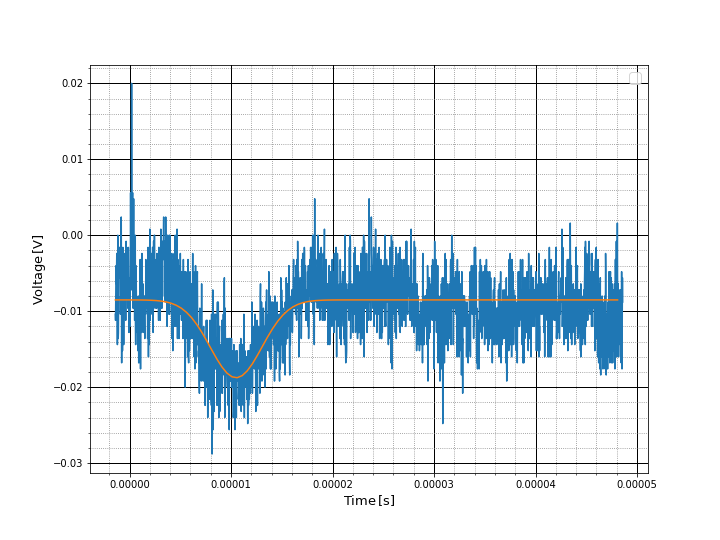
\includegraphics[scale=0.5]{Bild/A1}
	\centering
	\caption[Gaußfit an Messung bei Konst. Abstand]{Gaußfit an die Messungen der Elektronenwolken bei Konstantem Abstand von $3.6$\,mm und einer Spannung von $-48.0$\,V}
\end{figure}

%Lange Messungen

\begin{figure}[ht]
	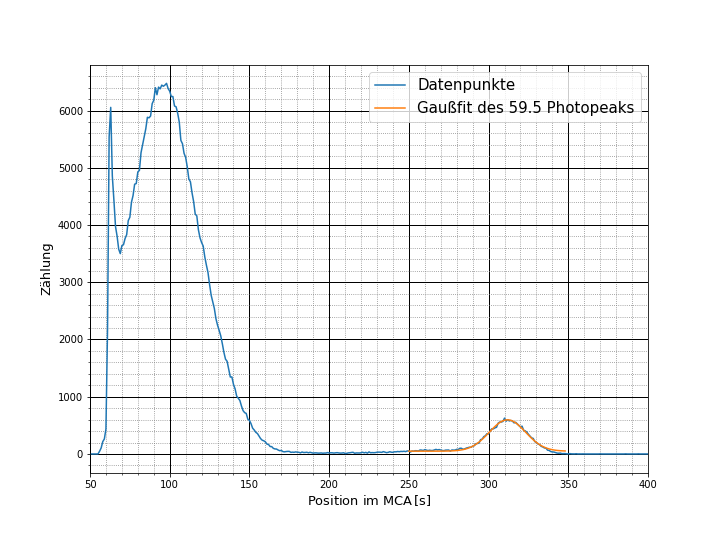
\includegraphics[scale=0.5]{Bild/ASg}
	\centering
	\caption{Gesamtes Spektrum von Americium mit Silizium aufgenommen.}
\end{figure}
\begin{figure}[ht]
	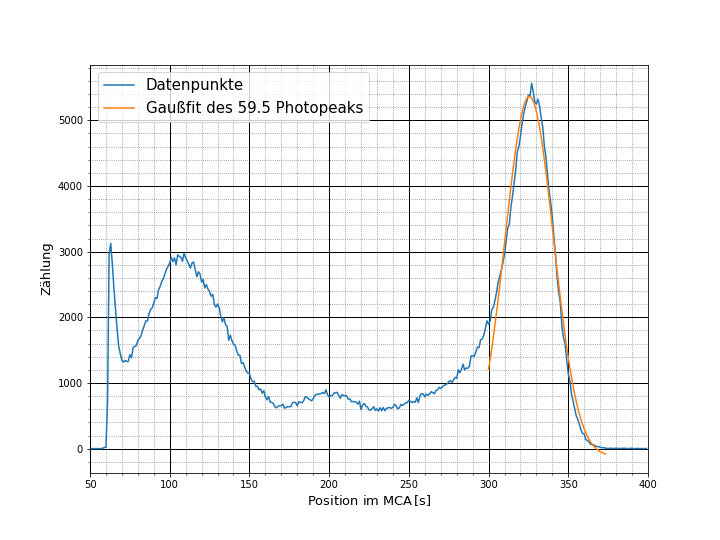
\includegraphics[scale=0.5]{Bild/ACg}
	\centering
	\caption{Gesamtes Spektrum von Americium mit CdTe aufgenommen.}
\end{figure}
\begin{figure}[ht]
	\includegraphics[scale=0.5]{Bild/CSg}
	\centering
	\caption{Gesamtes Spektrum von Cobalt mit Silizium aufgenommen.}
\end{figure}
\begin{figure}[ht]
	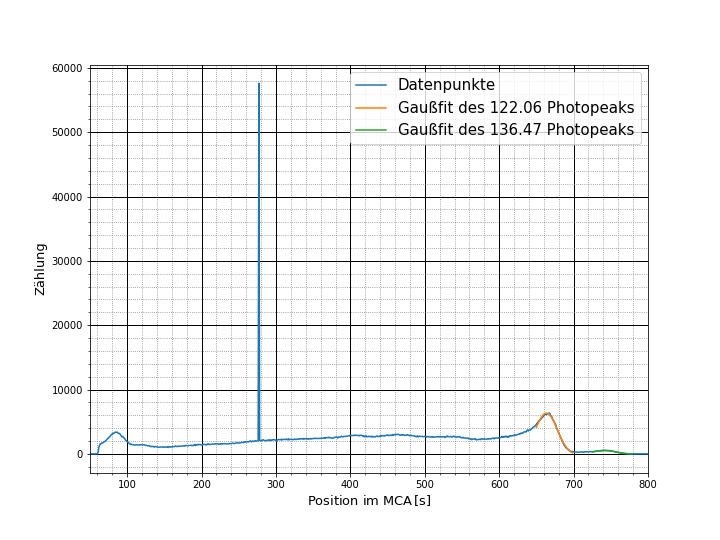
\includegraphics[scale=0.5]{Bild/CCg}
	\centering
	\caption{Gesamtes Spektrum von Cobalt mit CdTe aufgenommen.}
\end{figure}